\documentclass[border=10pt]{standalone}

\usepackage{tikz}
\usepackage{tikzsymbols}
\usetikzlibrary{calc,patterns,shapes.geometric}

\def\centerarc[#1](#2)(#3:#4:#5){\draw[#1] ($(#2)+({#5*cos(#3)},{#5*sin(#3)})$) arc (#3:#4:#5);}

\begin{document}
	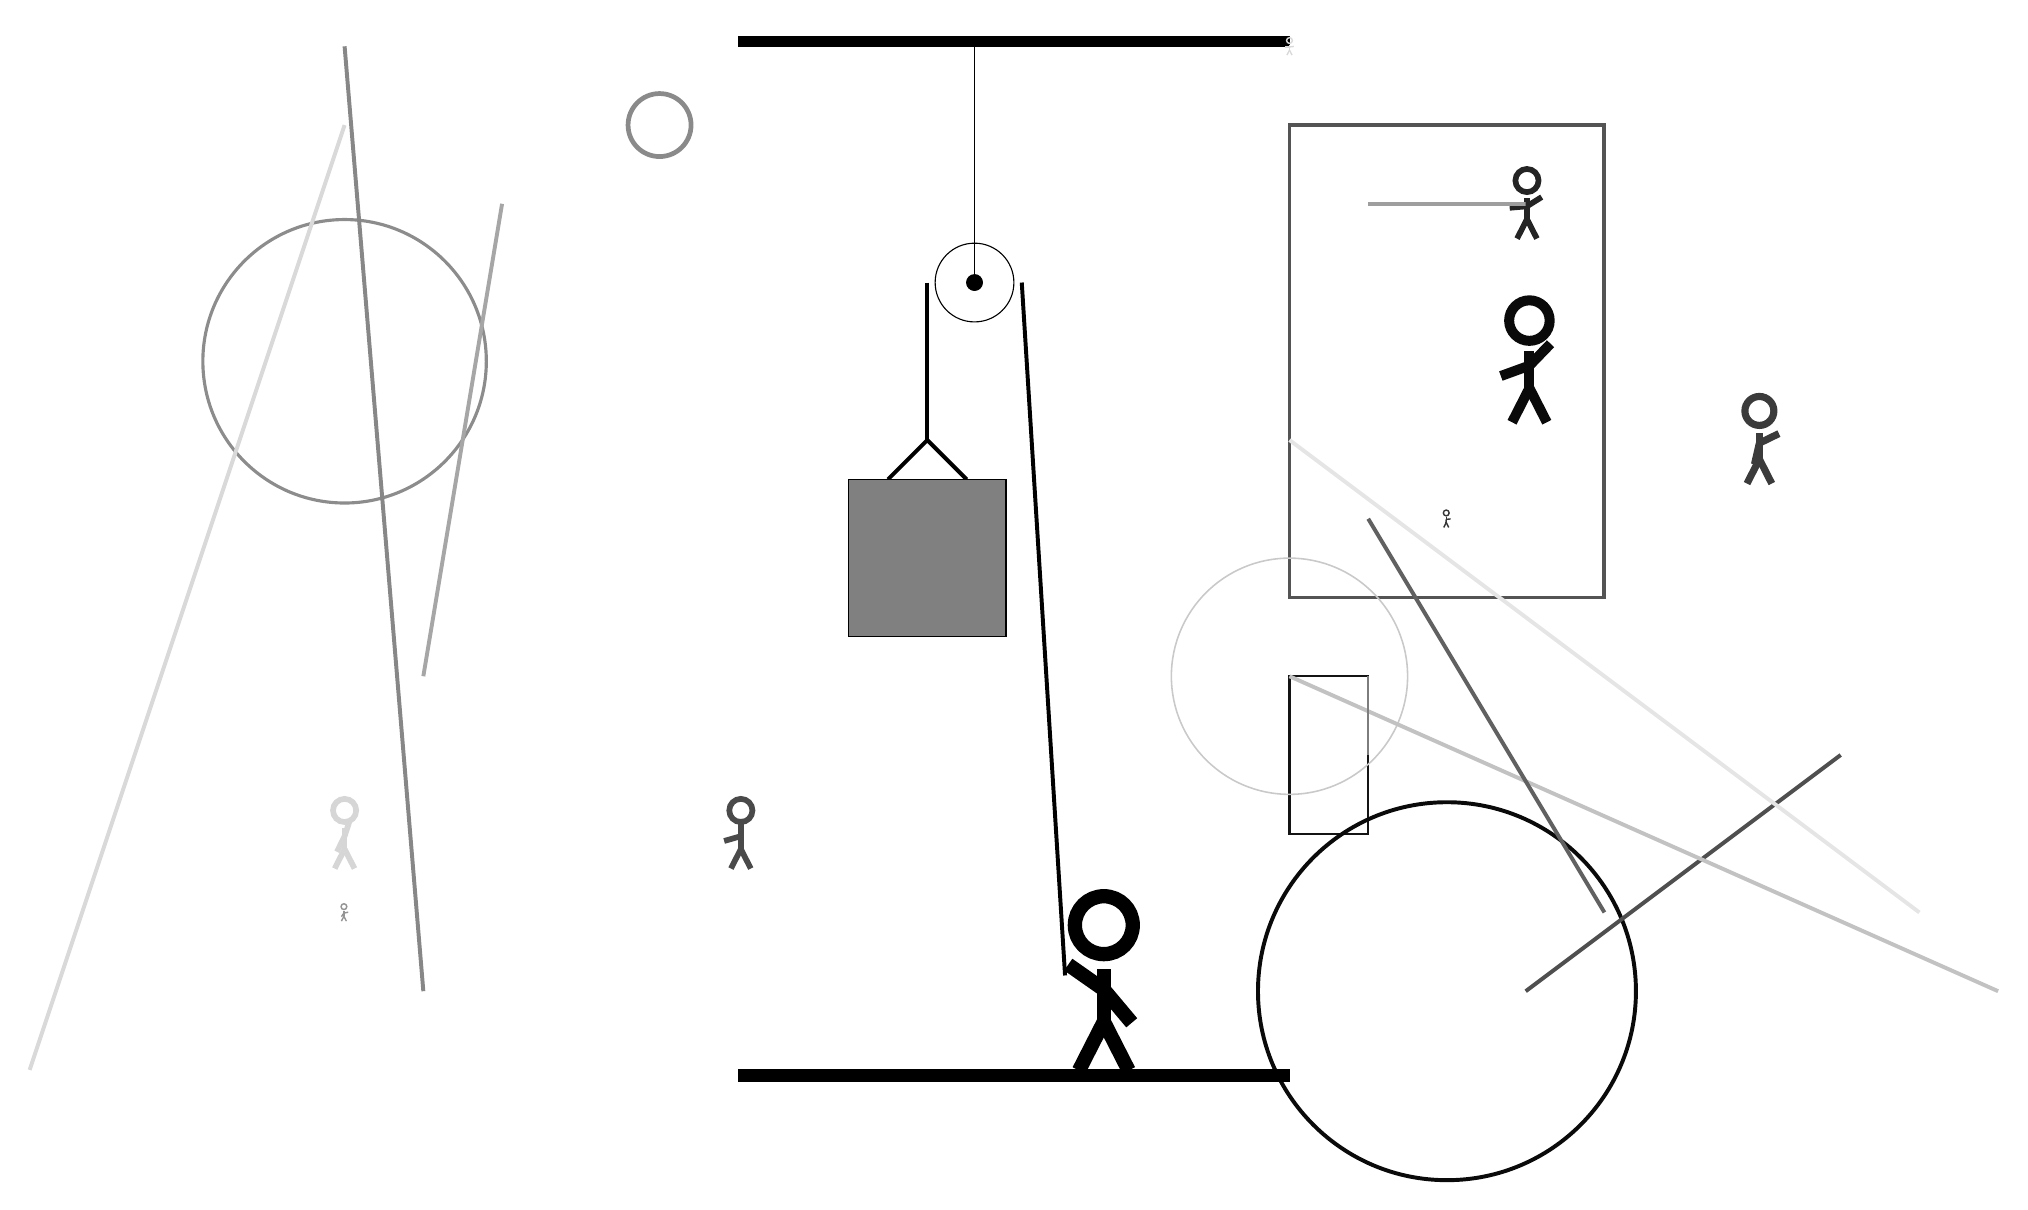
\begin{tikzpicture}
		%%%%% START %%%%%
		
		\draw[fill=black] (-2, 10) rectangle (5, 10.125);
		
		\draw (1, 7) circle (0.5);
		\draw[fill=black] (1, 7) circle (0.1);
		\draw (1, 10) -- (1, 7);
		
		\draw[line width=0.5mm] (-0.1, 4.5) -- (0.4, 5.0) -- (0.9, 4.5);
		\draw[fill=black!50] (-0.6, 4.5) rectangle (1.4, 2.5);
		
		\draw[line width=0.5mm] (0.4, 7) -- (0.4, 5.0);
		\centerarc[line width=0.5mm](1, 7)(0:180:0.6);
		\draw[line width=0.5mm](1.6, 7) -- (2.15, -1.8);
		
		\draw[line width=0.3mm, color=black!92] (5, 0) rectangle (6, 2);
		
		\node[line width=0.5mm, color=black!77] at (11, 5) {\Strichmaxerl[5][77][26]};
		\draw [line width=0.5mm, color=black!96](7, -2) circle (2.4);
		\node[line width=0.4mm, color=black!16] at (-7, 0) {\Strichmaxerl[4][64][72]};
		
		\draw[line width=0.5mm, color=black!69](8, -2) -- (12, 1);
		\draw[line width=0.5mm, color=black!67] (5, 9) rectangle (9, 3);
		
		\draw [line width=0.2mm, color=black!21](5, 2) circle (1.5);
		\node[line width=0.5mm, color=black!96] at (8, 6) {\Strichmaxerl[7][20][46]};
		\node[line width=0.5mm, color=black!86] at (8, 8) {\Strichmaxerl[4][5][32]};
		
		\draw [line width=0.4mm, color=black!45](-7, 6) circle (1.8);
		\draw[line width=0.5mm, color=black!47](-7, 10) -- (-6, -2);
		
		\draw[line width=0.5mm, color=black!24](5, 2) -- (14, -2);
		\draw[line width=0.5mm, color=black!38] (6, 8) rectangle (8, 8);
		\node[line width=0.4mm, color=black!15] at (5, 10) {\Strichmaxerl[1][0][7]};
		\draw [line width=0.3mm, color=black!49](-3, -1) circle (0.0);
		\draw[line width=0.5mm, color=black!10](5, 5) -- (13, -1);
		
		\draw [line width=0.6mm, color=black!46](-3, 9) circle (0.4);
		\node[line width=0.3mm, color=black!71] at (-2, 0) {\Strichmaxerl[4][16][89]};
		\node[line width=0.7mm, color=black!42] at (-7, -1) {\Strichmaxerl[1][55][12]};
		\draw[line width=0.5mm, color=black!62](9, -1) -- (6, 4);
		\draw[line width=0.5mm, color=black!35](-5, 8) -- (-6, 2);
		\draw[line width=0.3mm, color=black!51] (6, 1) rectangle (6, 2);
		\node[line width=0.4mm, color=black!79] at (7, 4) {\Strichmaxerl[1][84][6]};
		\draw[line width=0.5mm, color=black!15](-7, 9) -- (-11, -3);
		
		\node at (2.6, -1.9) {\Strichmaxerl[10][-35][-50]};
		
		\draw[fill=black] (-2, -3) rectangle (5, -3.15);
		
		%%%%% END %%%%%
	\end{tikzpicture}
\end{document}